\begin{figure}[htbp]
  \centering
  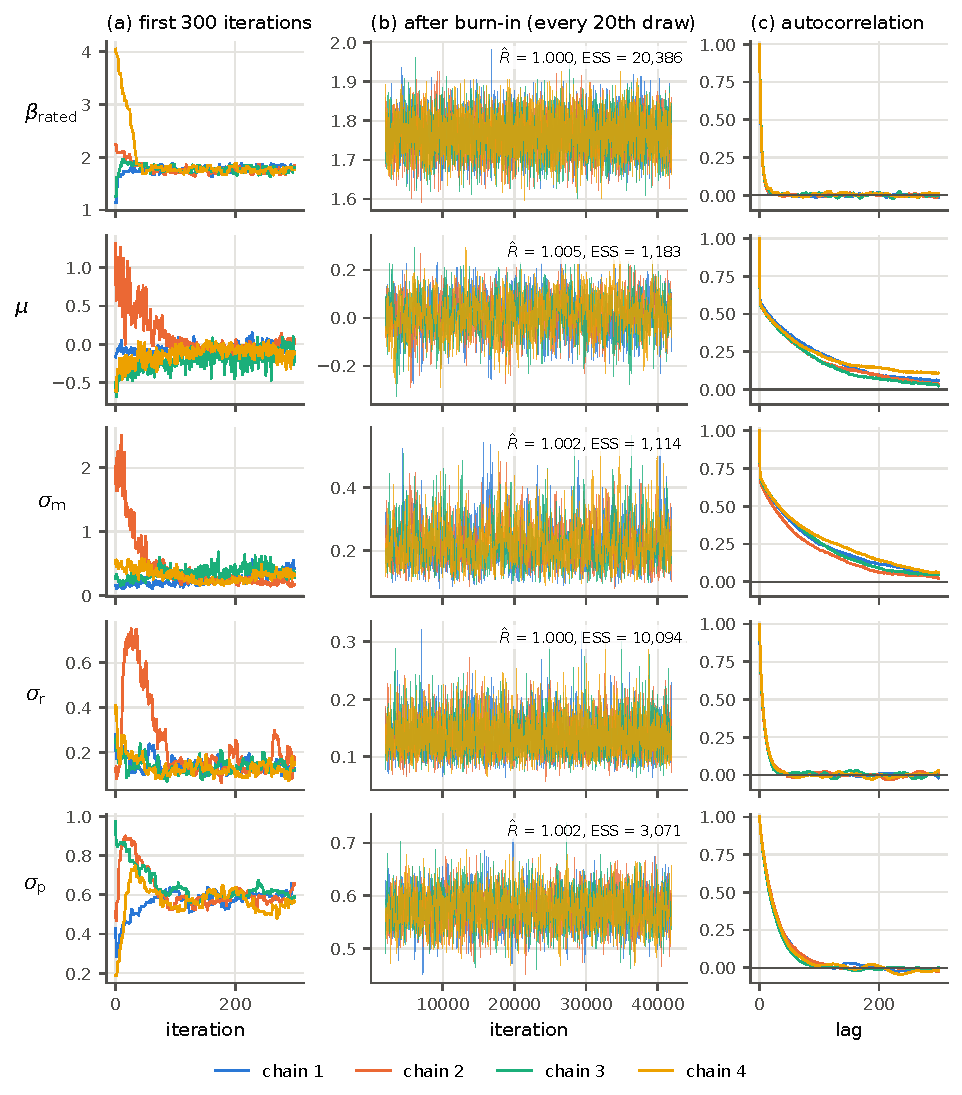
\includegraphics[width=\linewidth]{trace_full.pdf}
  \caption{Convergence of the sampler of the final model on the real data: 4 chains started from points drawn from the prior. (a): the first 300 iterations; (b): the 40,000 iterations kept per chain after a burn-in of 2,000, with the split-$\hat R$ and the effective sample size (ESS) of the four chains together; (c): autocorrelation of each chain after burn-in. The slope $\beta$ mixes fast. The spreads of the replies and of the players, which have moves that rescale their whole level at once, reach an ESS of 10,094 and 3,071; $\mu$ and $\sigma_{\mathrm{m}}$, learned from only 20 first moves, are the slowest, with an ESS of 1,183 and 1,114, still enough for small Monte Carlo errors.}
  \label{fig:trace_full}
\end{figure}
